\documentclass[a4paper,11pt]{article}
\usepackage[utf8]{inputenc}
\usepackage[T1]{fontenc}
\usepackage{graphicx}
\usepackage[T2A]{fontenc}
\usepackage[utf8]{inputenc}
\usepackage[english]{babel}
\usepackage{extsizes}
\usepackage{indentfirst}
\usepackage{fancyhdr}
\usepackage{geometry}
\usepackage{amsthm}
\usepackage{amsfonts}
\usepackage{mathtools}
\usepackage{graphicx}
\usepackage{wrapfig}
\usepackage{caption}
\usepackage{amssymb}
\usepackage{booktabs}
\usepackage{dsfont}
\usepackage[toc,page]{appendix}
\usepackage[export]{adjustbox}
\usepackage[percent]{overpic}

\theoremstyle{plain}
\newtheorem{thm}{Theorem}
\newtheorem{lmm}[thm]{Lemma}
\newtheorem{crlr}[thm]{Corollary}

\theoremstyle{definition}
\newtheorem{defn}[thm]{Definition}
\newtheorem{exmp}[thm]{Example}
\newtheorem{rmrk}[thm]{Remark}
\newtheorem{asmp}[thm]{Assumption}
\newtheorem{prps}[thm]{Proposition}
\newtheorem{cond}[thm]{Conditions}


\renewenvironment{proof}{{\scshape Proof:}}{}

\renewcommand{\theenumi}{\roman{enumi}}
\renewcommand{\labelenumi}{(\theenumi)}

\newcommand{\ME}{\mathbb{E}}
\newcommand{\MR}{\mathbb{R}}
\newcommand{\MP}{\mathbb{P}}
\newcommand{\MN}{\mathbb{N}}
\newcommand{\Var}{\mathrm{Var}}
\newcommand{\Cov}{\mathrm{Cov}}
\newcommand{\diag}{\mathrm{diag}}
\newcommand{\tr}{\mathrm{tr}}
\newcommand{\convdistr}{\xrightarrow{\mathcal{L}}}
\newcommand{\convprob}{\xrightarrow{\MP}}
\newcommand{\define}[1]{\textit{\textbf{#1}}}
%\graphicspath{{./chapters/chapter01/}}
%opening
\title{On the estimation of integrated covariance matrices of high dimensional diffusion processes}
\author{Aleksandr Samarin}
\date{August 2017}

\begin{document}
	
	\maketitle
	
	\begin{abstract}
		(COPIED FROM THE PAPER) \\
		We consider the estimation of integrated covariance (ICV) matrices
		of high dimensional diffusion processes based on high frequency
		observations. We start by studying the most commonly used estimator,
		the realized covariance (RCV) matrix. We show that in the
		high dimensional case when the dimension p and the observation frequency
		n grow in the same rate, the limiting spectral distribution
		(LSD) of RCV depends on the covolatility process not only through
		the targeting ICV, but also on how the covolatility process varies in
		time. We establish a Marcenko–Pastur type theorem for weighted
		sample covariance matrices, based on which we obtain a Marcenko–
		Pastur type theorem for RCV for a class C of diffusion processes.
		The results explicitly demonstrate how the time variability of the
		covolatility process affects the LSD of RCV. We further propose
		an alternative estimator, the time-variation adjusted realized covariance
		(TVARCV) matrix. We show that for processes in class C, the
		TVARCV possesses the desirable property that its LSD depends
		solely on that of the targeting ICV through the Marcenko–Pastur
		equation, and hence, in particular, the TVARCV can be used to recover
		the empirical spectral distribution of the ICV by using existing
		algorithms
	\end{abstract}
	
	\section{Introduction}
	
	\[ \mathbf{X}_t = \big(X_t^{(1)}, \dots, X_t^{(p)}\big)^T \]
	\begin{equation} \label{X diffeq}
		d\mathbf{X}_t = \mathbf{\mu}_t dt + \Theta_td\mathbf{W}_t,
	\end{equation}
	where 
	\begin{itemize}
		\item $\mathbf{\mu}_t = (\mu_t^{(1)}, \dots, \mu_t^{(p)})^T$ is a $p-$dimensional drift process,
		\item $\Theta_t$ -- $p \times p$ \define{covolatility process},
		\item $\mathbf{W}_t$ -- $p$-dimensional standard Brownian motion.
	\end{itemize}
	
	\begin{defn} \
		\begin{enumerate}
			\item The \define{integrated covariance matrix (ICV)} is
			\[\Sigma_p := \int_0^1\Theta_t \Theta_t^T dt.\]
			For $p=1$ ICV is called \define{integrated volatility}.
			\item Set time points $\tau_{n, \ell}$. Then \define{realized covariance (RCV)} is
			\begin{equation} \label{RCV}
				\Sigma_p^{RCV} := \sum_{\ell=1}^{n}\Delta \mathbf{X}_\ell(\Delta \mathbf{X}_\ell)^T,
			\end{equation}
			where 
			\[ \Delta \mathbf{X}_\ell :=
			\begin{pmatrix}
			\Delta X_\ell^{(1)} \\
			\vdots \\
			\Delta X_\ell^{(p)}
			\end{pmatrix}
			=
			\begin{pmatrix}
			X_{\tau_{n,\ell}}^{(1)} - X_{\tau_{n, \ell-1}}^{(1)} \\
			\vdots \\
			X_{\tau_{n,\ell}}^{(p)} - X_{\tau_{n, \ell-1}}^{(p)}
			\end{pmatrix}. \]
			For $p=1$ RCV is called \define{realized volatility}.
			\item Let $\{\lambda_j:j=1,\dots, p\}$ be set of eigenvalues of ICV, then
			\[F^{\Sigma_p}(x) := \frac{\#\{j:\lambda_j \leq x\}}{p}, \quad x \in \MR, \]
			is called \define{empirical spectral distribution (ESD)}.
		\end{enumerate}
	\end{defn}
	
	
	Let us set
	\[ \Theta_t^0 = \sqrt{\int_0^1\Theta_s \Theta_s^T ds} \quad \forall t \in [0, 1] \]
	and corresponding matrix $\mathbf{X}_t^0$, such that
	\[ d\mathbf{X}_t^0 = \Theta_t^0d\mathbf{W}_t. \]
	Note that $\mathbf{X}_t$ and $\mathbf{X}_t^0$ share the same ICV matrix:
	\[ \Sigma_p^0 :=  \int_0^1\Theta_t^0 {\Theta_t^0}^T dt = \int_0^1 dt \int_0^1\Theta_s \Theta_s^T ds = \Sigma_p.  \]
	
	\section{Marchenko-Pastur law}
	
	\begin{prps} [Theorem 1.1 of Silverstein (1995)] \label{MP law} \
		\begin{enumerate}
			\item for $p = 1, 2, \dots$ and for $1 \leq \ell \leq n$, $\mathbf{Z}_\ell^{(p)} = (Z_\ell^{(p,j)})_{1 \leq j \leq p}$ with $Z_\ell^{(p,j)}$ i.i.d. with mean 0 and variance 1;
			\item $n = n(p)$ with $y_n := p/n \rightarrow y > 0$ as $p \rightarrow \infty$;
			\item $\Sigma_p$ is a (possibly random) nonnegative definite $p \times p$ matrix such that its ESD $F^{\Sigma_p}$ converges a.s. in distribution to a probability distribution $H$ on $[0,\infty)$ as $p \rightarrow \infty$;
			\item $\Sigma_p$ and $\mathbf{Z}_\ell^{(p)}$ are independent.
		\end{enumerate}
		Let $\Sigma_p^{1/2}$ be the (nonnegative) square root matrix of $\Sigma_p$ and 
		\[S_p:= \frac{1}{n} \sum_{\ell=1}^{n} \Sigma_p^{1/2} \mathbf{Z}_\ell^{(p)}(\mathbf{Z}_\ell^{(p)})^T \Sigma_p^{1/2}.\]
		Then a.s. the ESD of $S_p$ converges in distribution to a probability distribution $F$, which is determined by $H$ in that its Stieltjes transform
		\[ m_F(z):=\int_{\lambda \in \MR} \frac{1}{\lambda - z} dF(\lambda), \quad z \in \mathbb{C}_+ := \{ z \in \mathbb{C} : \Im(z)>0 \} \]
		solves the equation
		\begin{equation}
		m_F(z) = \int_{\tau \in \MR} \frac{1}{\tau (1-y(1+zm_F(z))) - z } dH(\tau).
		\end{equation}
	\end{prps}
	
	Note that if $y \rightarrow 0$ limiting distribution function $F$ of $S_p$ matches limiting distribution function $H$ of $\Sigma_p$.
	
	In the special case when $\Sigma_p = \sigma^2 \mathbb{I}_{p \times p}$, where $\mathbb{I}_{p \times p}$ is the $p \times p$ identity matrix, the LSD $F$ can be explicitly expressed as follows.
	
	\begin{prps}[see, e.g., Theorem 2.5 in Bai (1999)]
		Suppose that $\mathbf{Z}_\ell^{(p)}$'s are as in the previous proposition, and $\Sigma_p = \sigma^2 \mathbb{I}_{p \times p}$ for some $\sigma^2>0$. Then the LSD $F$ has density
		\[ f(x) = \Big(1-\frac{1}{y}\Big)_+\delta_0(x) + \frac{1}{2 \pi \sigma^2 xy} \sqrt{(b-x)(x-a)} \mathbf{1}_{[a,b]}(x), \]
		where 
		\[ a = \sigma^2(1-\sqrt{y})^2 \quad \text{and} \quad b = \sigma^2(1+\sqrt{y})^2, \]
		and $\delta_0(x)$ is a Dirac delta function.
	\end{prps}
	The LSD $F$ in this proposition is called the Marchenko-Pastur law with ratio index $y$ and scale index $\sigma^2$, and will be denoted by $\mathcal{MP}(y, \sigma^2)$.
	\begin{figure}
		\begin{center} \centering
			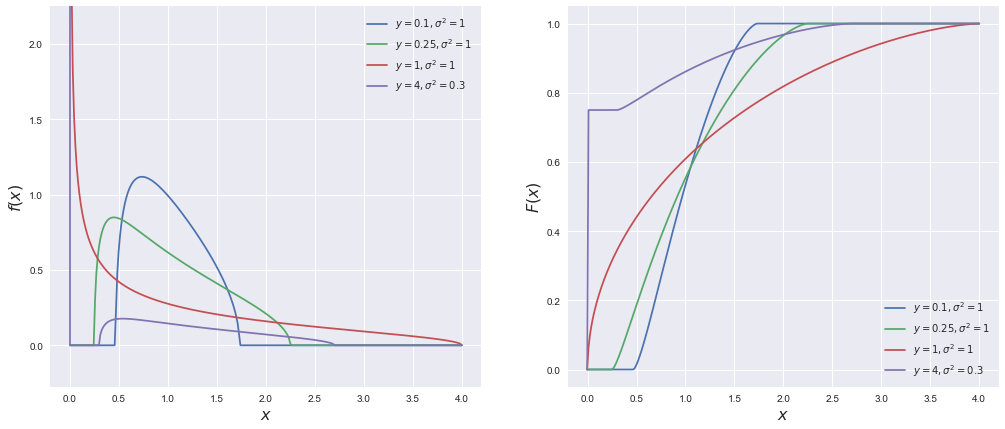
\includegraphics[scale=0.4]{MP}
			\caption{Marchenko-Pastur law}
		\end{center}
	\end{figure}
	
	
	\begin{thm}[Weyl's Monotonicity Theorem]
		Suppose $A$ and $B$ are symmetric, $p \times p$ matrices. Let $\lambda_i(A)$ be the $i$-th largest eigenvalue of $A$. If $A \preceq B$, then $\lambda_i(A) \leq \lambda_i(B)$ for all $i$, or, equivalently
		\[ F^B(x) \leq F^A(x) \quad \forall x \geq 0. \]
    \end{thm}
    \begin{proof}
    	Corollary 4.3.3 in Horn and Johnson (1990)
    \end{proof}
		
	\begin{prps}
		Suppose that for all $p$, $\mathbf{X}_t=\mathbf{X}_t^{(p)}$ is a $p$-dimensional process satisfying
		\begin{equation}
		d \mathbf{X}_t = \gamma_t d\mathbf{W}_t, \quad t \in [0, 1],
		\end{equation}
		where $\gamma_t > 0$ is a nonrandom (scalar) c$\grave{a}$dl$\grave{a}$g process. Let $\sigma^2 = \int_0^1 \gamma_t^2 dt$ and so that the ICV matrix $\Sigma_p = \sigma^2 \mathbb{I}_{p \times p}$. Assume further that the observation times $\tau_{n,\ell}$ are equally spaced, that is, $\tau_{n, \ell} = \ell / n$, and that the RCV matrix $\Sigma_p^{RCV}$ is defined by \eqref{RCV}. Then so long as $\gamma_t$ is not constant on $[0, 1)$, for any $\varepsilon > 0$, there exists $y_c = y_c(\gamma, \varepsilon) > 0$ such that if $\lim p/n = y \geq y_c$,
		\begin{equation}
			\limsup F^{\Sigma_p^{RCV}}(b(y)+\sigma^2\varepsilon) < 1 \quad a.s.
		\end{equation}
		In particular, $F^{\Sigma_p^{RCV}}$ doesn't converge to the Marchenko-Pastur law $\mathcal{MP}(y, \sigma^2)$.
    \end{prps}
    
    \begin{proof}
    	By assumption if $\gamma_t$ is non-contant, there exists $\delta > 0$ and an interval $[c, d] \subseteq [0, 1] $ such that
    	\[ \gamma_t \geq \sigma(1+\delta) \quad \forall t \in [c, d]. \]
    	Therefore, if $\big[ \frac{\ell - 1}{n}, \frac{\ell}{n} \big] \subseteq [c, d] $ for some $1 \leq \ell \leq n$, then
    	\[ \Delta \mathbf{X}_\ell (\Delta \mathbf{X}_\ell )^T \stackrel{d}{=} \int_{(\ell-1)/n}^{\ell/n} \gamma_t^2 dt \cdot \mathbf{Z}_\ell(\mathbf{Z}_\ell)^T \succeq \frac{(1+\delta)^2}{n} \sigma^2 \mathbf{Z}_\ell(\mathbf{Z}_\ell)^T,  \]
    	where $\mathbf{Z}_\ell = (Z_\ell^{(1)}, \dots , Z_\ell^{(p)})^T$ consists of independent standard normals. Hence, if we let $ J_n = \big\{ \ell: \big[ \frac{\ell - 1}{n}, \frac{\ell}{n} \big] \subseteq [c, d] \big\} $ and
    	\[ \Gamma_p = \sum_{\ell \in J_n} \Delta \mathbf{X}_\ell (\Delta \mathbf{X}_\ell )^T, \quad \Lambda_p = \frac{\sigma^2}{n(d-c)} \sum_{\ell \in J_n} \mathbf{Z}_\ell (\mathbf{Z}_\ell )^T,  \]
    	then for any $x \geq 0$, by Weyl's Monotonicity Theorem,
    	\[
    	F^{\Sigma_p^{RCV}}(x) \leq F^{\Gamma_p}(x) \leq F^{\Lambda_p}\bigg(\frac{x}{(1+\delta)^2(d-c)}\bigg).
    	\]
	    Now note that $\# J_n \sim (d-c)n$, hence if $p/n \rightarrow y$, by Proposition \ref{MP law}, $F^{\Lambda_p}$ will converge a.s. to the Marchenko-Pastur law with ratio index $y'=\frac{y}{d-c}$ and scale index $\sigma^2$.
	    By the formula of $b(\cdot)$ in Marchenko-Pastur density
	    \[
	    \begin{aligned}
	    (1+\delta)^2(d-c)b(y') &=(1+\delta)\sigma^2 \cdot (1+\delta)(d-c)(1+2\sqrt{y'}+y') \\
	    & =(1+\delta)\sigma^2 \cdot (1+\delta)(d-c + 2\sqrt{(d-c)y} + y) \\
	    & := (1+\delta)\sigma^2 \cdot  g(y).
	    \end{aligned}
	    \]
	    Note that the $g(y)$ has a linear growth in $y$ with coefficient $1+\delta$. Hence, for any $\varepsilon > 0$, there exists $y_c > 0$, such that for all $y \geq y_c$
	    \[ g(y) \geq (1+\sqrt{y})^2+\varepsilon,  \]
	    that is,
	    \[ (1+\delta)^2(d-c)b(y') \geq (1+\delta) \sigma^2 \cdot ((1+\sqrt{y})^2+\varepsilon) = (1+\delta)(b(y)+\sigma^2\varepsilon)  \]
	    or, equivalently,
	    \[ \frac{b(y) + \sigma^2\varepsilon}{(1+\delta)^2(d-c)} \leq \frac{b(y')}{1+\delta}. \]
	    Therefore, when the above inequality holds,
	    \[\limsup F^{\Sigma_p^{RCV}}(b(y) + \sigma^2\varepsilon) \leq \limsup F^{\Lambda_p}\bigg(\frac{b(y')}{1+\delta}\bigg) < 1. \]
    \end{proof}
    
    \section{Limiting theorems for non-constant covolatility process}
    
    \begin{defn} \
    	\begin{enumerate}
    		\item Suppose that $\mathbf{X}_t$ is a $p$-dimensional process satisfying \eqref{X diffeq}, and $\Theta_t$ is c$\grave{a}$dl$\grave{a}$g. We say that $\mathbf{X}_t$ belongs to \define{class $\mathcal{C}$} if, almost surely, there exist $\gamma_t: [0, 1] \mapsto \MR$ and $\Lambda$ a $p \times p$ matrix satisfying $\tr(\Lambda \Lambda^T) = p$ such that 
    		\begin{equation} \label{class C cov}
    		\Theta_t = \gamma_t \Lambda.
    		\end{equation}
    		Observe that if \eqref{class C cov} holds, then the ICV matrix $\Sigma_p = \int_{0}^{1} \gamma_t^2 dt \cdot \Lambda \Lambda^T$.
    		\item Suppose that a diffusion process $\mathbf{X}_t$ belongs to class $\mathcal{C}$. We define \define{time-variation adjusted realized covariance (TVARCV) matrix} as follows:
    		\begin{equation} \label{TVARCV}
    		\widehat{\Sigma}_p := \frac{\tr \big( \Sigma_p^{RCV} \big) }{n} \sum_{\ell = 1}^{n} \frac{\Delta \mathbf{X}_\ell (\Delta \mathbf{X}_\ell)^T}{\| \Delta \mathbf{X}_\ell \|_2^2} = \frac{\tr \big( \Sigma_p^{RCV} \big) }{p} \widetilde{\Sigma}_p,
    		\end{equation}
    		where
    		\begin{equation} \label{Sigma_tilde}
    		\widetilde{\Sigma}_p := \frac{p}{n} \sum_{\ell = 1}^{n} \frac{\Delta \mathbf{X}_\ell (\Delta \mathbf{X}_\ell)^T}{\| \Delta \mathbf{X}_\ell \|_2^2}.
    		\end{equation}
    	\end{enumerate}
    \end{defn}
    
    \begin{rmrk}
    	Let us explain $\widetilde{\Sigma}_p$. Consider the simplest case when $\mu_t = 0$, $\gamma_t$ deterministic, $\Lambda_t = \mathbb{I}_{p \times p}$, and $\tau_{n,\ell} = \ell / n$, $\ell = 0, 1, \dots, n$. In this case,
    	\[ \Delta \mathbf{X}_\ell = \sqrt{\int_{(\ell - 1)/n}^{\ell / n} \gamma_t^2 dt }\cdot \frac{\mathbf{Z}_\ell}{\sqrt{n}}, \]
    	where $\mathbf{Z}_\ell = (Z_\ell^{(1)}, \dots, Z_\ell^{(p)})^T$ is a vector of i.i.d. standard normal random variables. Hence,
    	\[ \frac{\Delta \mathbf{X}_\ell (\Delta \mathbf{X}_\ell)^T}{\| \Delta \mathbf{X}_\ell \|_2^2} = \frac{\mathbf{Z}_\ell \mathbf{Z}_\ell^T}{\|  \mathbf{Z}_\ell \|_2^2}. \]
    	However, as $p \rightarrow \infty$, $\| \mathbf{Z}_\ell \|_2^2 \sim p$, hence
    	\[ \widetilde{\Sigma}_p \sim \frac{\sum_{\ell = 1}^{n}\mathbf{Z}_\ell \mathbf{Z}_\ell^T}{n}, \]
    	the latter being the usual sample covariance matrix.
    \end{rmrk}
    
    
\end{document}
